\documentclass[12pt, titlepage]{article}

\usepackage{booktabs}
\usepackage{xr-hyper}
\usepackage{tabularx}
\usepackage{graphicx}
\usepackage{listings}
\graphicspath{{../../src/TestCase/}}
\usepackage{hyperref}
\hypersetup{
    colorlinks,
    citecolor=black,
    filecolor=black,
    linkcolor=red,
    urlcolor=blue
}

%% Comments

\usepackage{color}

\newif\ifcomments\commentstrue

\ifcomments
\newcommand{\authornote}[3]{\textcolor{#1}{[#3 ---#2]}}
\newcommand{\todo}[1]{\textcolor{red}{[TODO: #1]}}
\else
\newcommand{\authornote}[3]{}
\newcommand{\todo}[1]{}
\fi

\newcommand{\wss}[1]{\authornote{blue}{SS}{#1}}
\newcommand{\an}[1]{\authornote{magenta}{Author}{#1}}

\externaldocument{../TestPlan/TestPlan}
\externaldocument{../SRS/SRS}
\newcommand{\progname}{SpectrumImageAnalysisPy}

\newcounter{reqnum} %Requirement Number
\newcommand{\rthereqnum}{P\thereqnum}
\newcommand{\rref}[1]{R\ref{#1}}

\begin{document}

\title{Test Report: SpectrumImageAnalysisPy} 
\author{Isobel Bicket}
\date{\today}
	
\maketitle

\pagenumbering{roman}

\section{Revision History}

\begin{tabularx}{\textwidth}{p{4cm}p{2cm}X}
\toprule {\bf Date} & {\bf Version} & {\bf Notes}\\
\midrule
December 18, 2017 & 1.0 & Initial draft\\
\bottomrule
\end{tabularx}

~\newpage

\section{Symbols, Abbreviations and Acronyms}
See \hyperref[Doc:SRS]{SRS} document for further definitions.\\

\renewcommand{\arraystretch}{1.2}
\begin{tabular}{l l} 
  \toprule		
  \textbf{symbol} & \textbf{description}\\
  \midrule 
  RMS & Root Mean Square\\
  SNR & Signal-to-Noise Ratio\\
  T & Test\\
  \bottomrule
\end{tabular}\\


\newpage

\tableofcontents

\listoftables %if appropriate

\listoffigures %if appropriate

\newpage

\pagenumbering{arabic}

This document details the results of the testing detailed in the
\hyperref[Doc:TestPlan]{Test Plan}, for the code \progname, which can be found,
along with the other documentation, on
\url{https://github.com/icbicket/SpectrumImageAnalysisPy/tree/SpectrumImageAnalysisPy_dev}. 
Data and results from testing can be found under 
\url{/home/isobel/Documents/McMaster/PythonCodes/DataAnalysis/src/TestCase}.

\section{Functional Requirements Evaluation}
In this section, the testing for each of the functional requirements is
addressed. Some testing is still in progress and will be completed at a later
date.
\subsection{\rref{R_SI_inputs}: SI Inputs}
Some \hyperref[sec:UnitTest]{unit testing} has been performed for error checking
on initializing a spectrum image. More remains to be done.

\subsection{\rref{R_spectrum_inputs}: Spectrum Inputs}
Testing remains to be done.

\subsection{\rref{R_Input_dimension}: Input Verification}
Some \hyperref[sec:UnitTest]{unit testing} has been performed for error checking
on initializing a spectrum image. More remains to be done.

\subsection{\rref{R_SI_slicing}: Slice (1D) SI and extract Image}
Some \hyperref[sec:UnitTest]{unit testing} has been performed on the 1D slice
module in Spectrum.

\subsection{\rref{R_SI_area}: Mask (2D) SI and extract Spectrum}
Testing remains to be done.

\subsection{\rref{R_deconvolution}: Richardson-Lucy Deconvolution}
The test data for testing the RMS error and SNR of the deconvolution algorithm
were obtained from Dr. E.P.Bellido and are the same datasets used in
\cite{bellido_toward_2014}. The inputs to the deconvolution function are shown
in Figure \ref{fig:RefSpec}. The original spectrum is simulated, with a narrow
Gaussian representing the zero loss peak. An experimental point spread function
was convolved with it to represent the blurring of the 'ideal' spectrum with the
point spread function of the CCD. Poisson noise was added to the result of this
convolution to imitate noise from the detector.

\begin{figure}[h]
    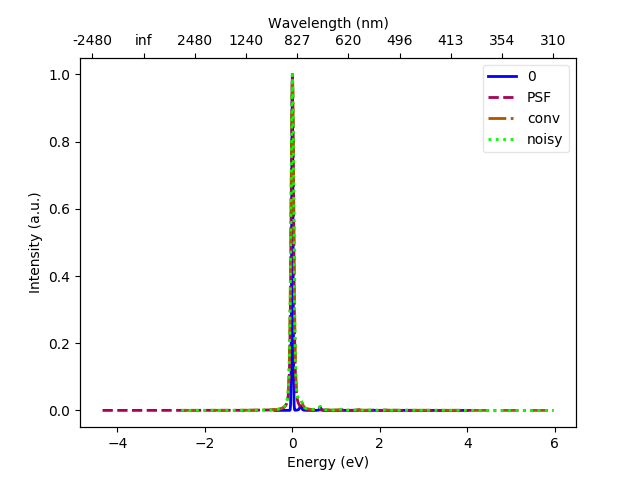
\includegraphics[scale=0.4]{Reference_spectra.png}
    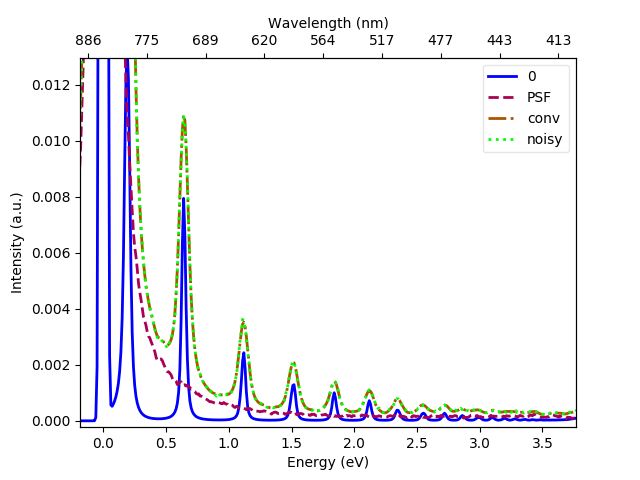
\includegraphics[scale=0.4]{Reference_spectra2.png}
    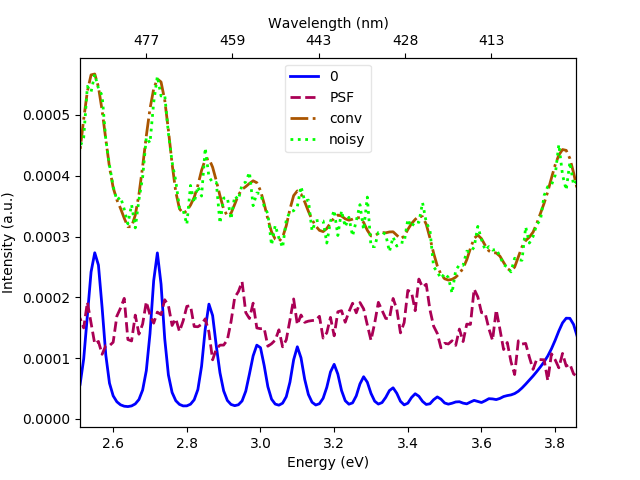
\includegraphics[scale=0.4]{Reference_spectra3.png}
    \caption{Original spectrum (0), Point spread function (PSF), the original
        spectrum convolved with the PSF (conv), and the original spectrum convolved
        with the PSF with Poisson noise added (noisy). Three images show three
        different regions of the spectrum.
        \label{fig:RefSpec}}
\end{figure}

The goal of deconvolution is to retrieve the original spectrum from the spectrum
convolved with the PSF. Up to 2000 iterations of the Richardson-Lucy
deconvolution algorithm have been performed on this dataset, using the
experimental point spread function, and the noisy convolved spectrum as inputs.
The results at several chosen values are shown in Figure \ref{fig:DeconvSpec}.
As the number of deconvolutions increases, the spectra quickly approach the
'ideal' spectrum (RL1, RL50). Further increments represent small benefits in the
approach to the 'ideal' spectrum (RL107-RL350). Using even more iterations
results in periodic artifacts starting to appear in the spectrum (RL1000,
RL2000), where small peaks appearing in between the main peaks can be seen and
grow larger with further iterations.

\begin{figure}[h]
    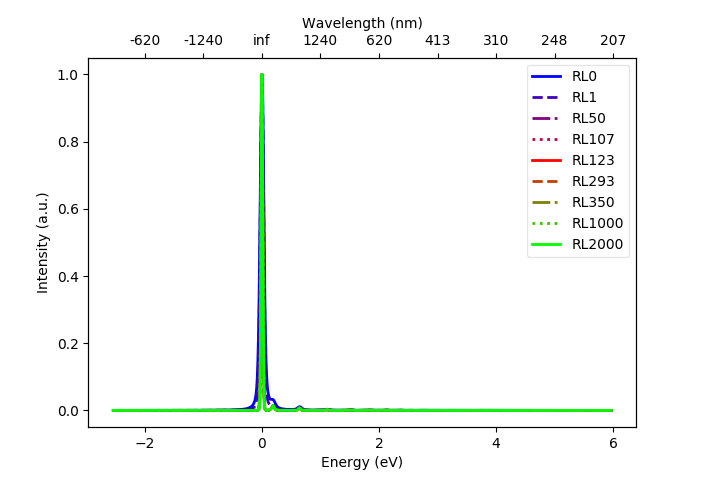
\includegraphics[scale=0.4]{Deconvolved_spectra_SimNoise3.png}
    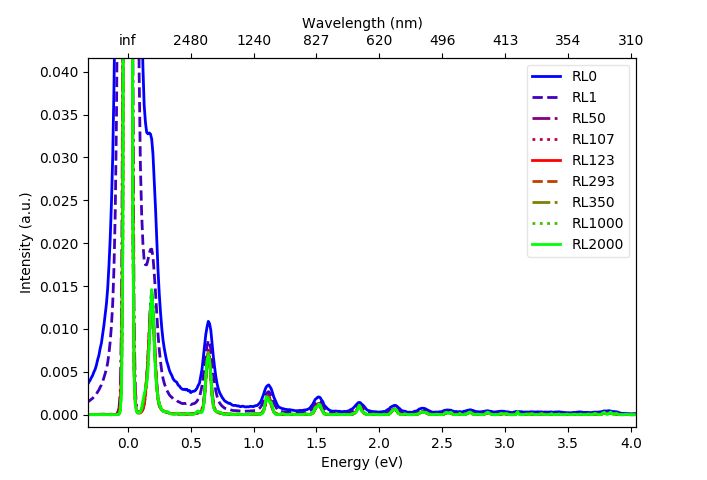
\includegraphics[scale=0.4]{Deconvolved_spectra_SimNoise3-2.png}
    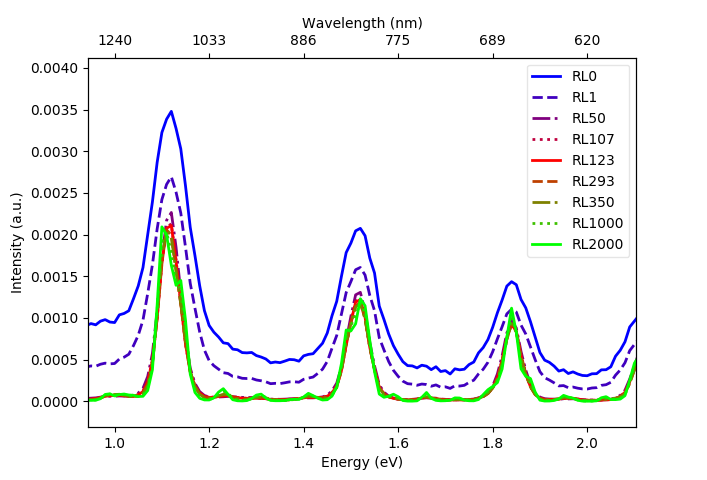
\includegraphics[scale=0.4]{Deconvolved_spectra_SimNoise3-3.png}
    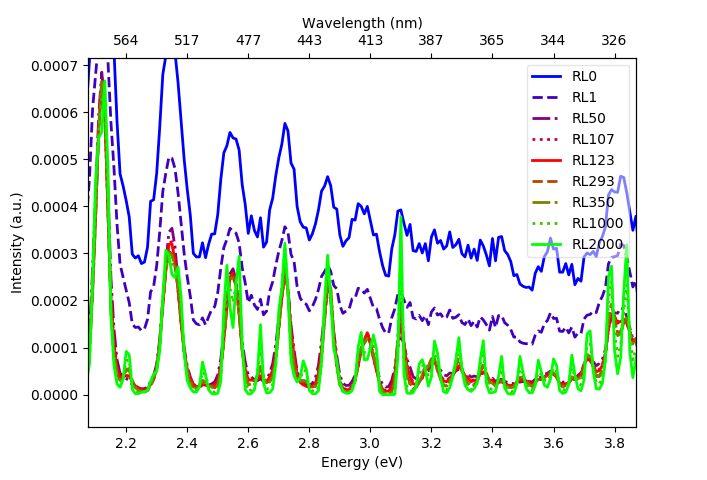
\includegraphics[scale=0.4]{Deconvolved_spectra_SimNoise3-4.png}
    \caption{Spectra deconvolved using the Richardson-Lucy algorithm. Different
        numbers of iterations were used, as shown in the legend (RL2000 = 2000
        iterations). Four images show different regions of the same plot.
    \label{fig:DeconvSpec}}
\end{figure}

To quantify the difference, the RMS error is plotted against the number of
iterations in \ref{fig:RMS}. There is at first a rapid decrease in the RMS
error, ending in a local minimum at around 100-120 iterations (the exact value
of the minimum depends on the noise added). Following this, the error increases
as the periodic artifacts begin to appear and grow larger. The minimum RMS error
at around 100-120 iterations represents about 0.12\% error.

\begin{figure}[h]
    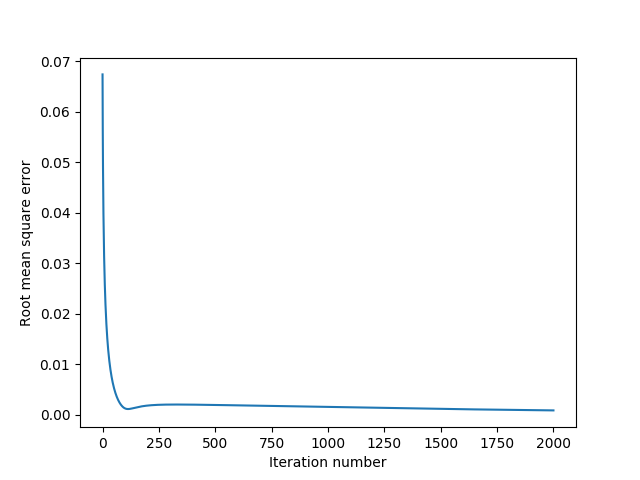
\includegraphics[scale=0.4]{rms_error-SimNoise3exp_PSF.png}
    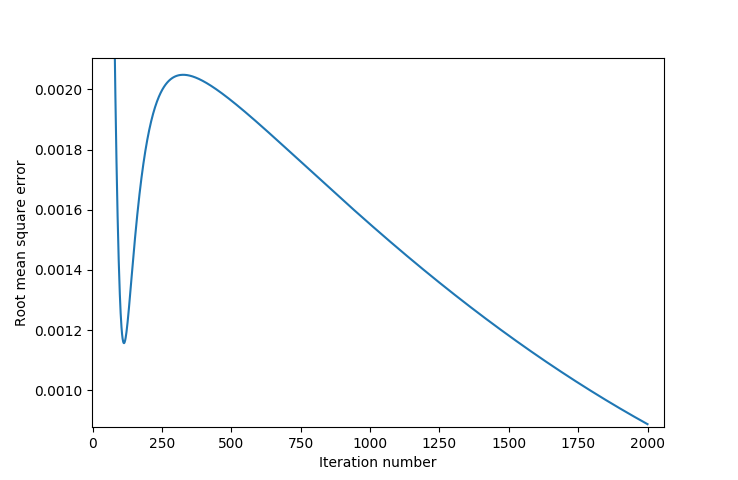
\includegraphics[scale=0.4]{rms_error-SimNoise3exp_PSF2.png}
    \caption{Root mean square error against number of RL deconvolution
        iterations performed. \label{fig:RMS}}
\end{figure}

To compare more directly with the data from Bellido \textit{et al.}
\cite{bellido_toward_2014}, the signal-to-noise ratio is plotted against the
number of iterations in Figure \ref{fig:SNR}. As was done by Bellido \textit{et
    al.}, the calculation for the SNR was split into two sections in the spectrum.
The SNR-ZLP section represents the SNR calculated within 0.1 eV of the zero loss
peak (at 0 eV), and the SNR-plasmon section represents the spectrum from 0.1 eV
to 4.0 eV (the 'plasmon region' of the spectrum). The SNR increases rapidly with
the first few iterations, followed by a peak at a similar value to the minimum
in the RMS error. Interestingly, the peak in SNR does not coincide exactly with
the RMS minimum, but is slightly offset in the number of iterations. There is
also a small difference between the SNR-ZLP and the SNR-plasmon peaks. After the
peak, the SNR-ZLP begins to increase. The ZLP is easily the strongest feature in
the spectrum: adding noise has very little effect on it and the SNR increases
with the number of iterations (after a local minimum). The SNR-plasmon, on the
other hand, has very little signal and the Poisson noise can easily dominate or
replace some of the smaller peaks. After the local maximum, the SNR-plasmon
begins to decrease and continues to decrease as the number of iterations
increases. Inspecting the results of the deconvolution in Figure
\ref{fig:DeconvSpec}, it is apparent that this is caused by the periodic
artifacts appearing between the peaks and the way that some of the peaks have
split into two peaks (\textit{e.g.}, near 2.6 eV).

These results are quite similar to those of Bellido \textit{et al.}, though not
exactly the same (likely due to the different Poisson noise used, since the
Poisson noise was generated independently for this test). Although it appears
that there is a further decrease in error and an increase in the ZLP-SNR with
large numbers of iterations, the results on the SNR-plasmon suggest that there
is an optimum number of iterations (dependent on the amount of noise) to balance
the RMS error and SNR for the region of interest, the plasmon region of the
spectrum; care must be taken with the number of iterations used, as higher
numbers can introduce extra spectrum peaks or emphasize the noise present. It
should be noted that this optimum number of iterations will be difficult to
determine in the experimental case, where the 'ideal' spectrum is not known and
the noise may be higher.

\begin{figure}[h]
    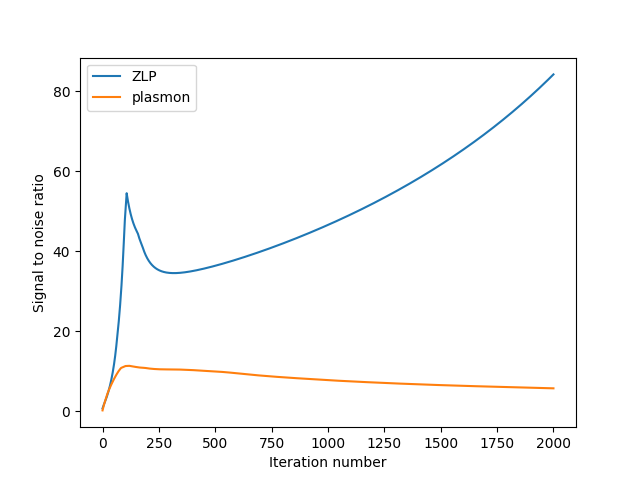
\includegraphics[scale=0.4]{snr-SimNoise3exp_PSF.png}
    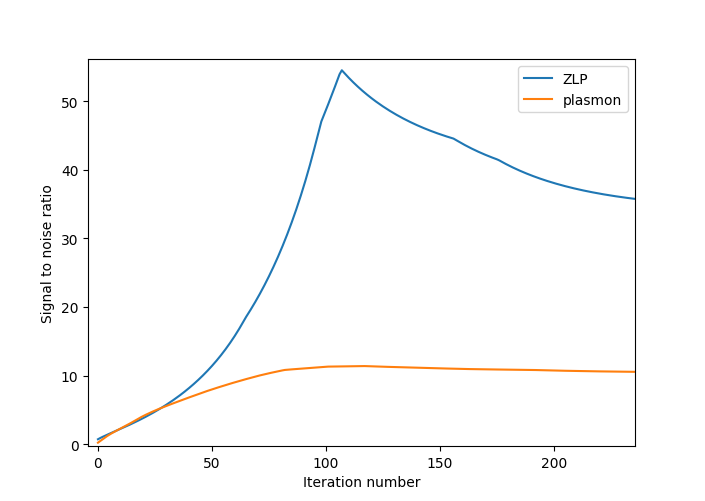
\includegraphics[scale=0.4]{snr-SimNoise3exp_PSF-2.png}
    \caption{Signal to noise ratio against number of iterations
        \label{fig:SNR}}
\end{figure}

\subsection{\rref{R_normalization}: Normalization}
Testing has not yet been performed for this functional requirement.

\subsection{\rref{R_background}: Background subtraction}
Testing has not yet been performed for this functional requirement.

\subsection{\rref{R_gain}: Gain Correction}
Testing has not yet been performed for this functional requirement.

\section{Nonfunctional Requirements Evaluation}

\subsection{Usability}
Testing has not yet been performed for this functional requirement. Tests for
the functional requirements and unit tests will be completed before asking users
to complete a survey on their experience.

\subsection{Performance}
Performance testing will be performed once unit tests and functional requirement
tests have been completed.

\section{Comparison to Existing Implementation}	
A comparison to the implementation in the HyperSpy python toolbox deconvolution
function will be performed in the future.

\section{Unit Testing}
\label{sec:UnitTest}
To date, partial unit testing has been performed on the following files:
\begin{itemize}
    \item Filenamer.py, used to name the files to be exported and avoid
    conflicts with already existing files).
    \item Spectrum.py, used to implement the Data 1D Spectrum module.
    \item SpectrumImage.py, used to implement the Data 3D Spectrum module
    \item ImagePlotter.py, implementing the Display 2D Image module.
\end{itemize}

The inputs, outputs, and procedure for each unit test can be found in each unit
test file. Coverage statistics for these files can be found in
\hyperref[ssec:StatCov]{Statement Coverage} and \hyperref[ssec:BrCov]{Branch
    Coverage}. As of the latest update, all unit tests were passing:

\begin{lstlisting}
    Ran 50 tests in 0.008s
    
    OK
\end{lstlisting}

\section{Changes Due to Testing}
\begin{itemize}
    \item A zero in the denominator during RL deconvolution now raises an exception
    \item Minor bug fixes
    \item Rewrite of the file naming program for exporting files
\end{itemize}
\section{Automated Testing}

\section{Trace to Requirements}

\begin{table}[H]
    \centering
    \begin{tabular}{|c|c|c|c|c|c|c|c|c|c|c|c|c|c|c|c|c|c|c|c|}
        \hline
        & & & & & \\
        \hline
             &  &  &  & & \\ \hline
                & &  & &  &  \\ \hline
                  &  & &  &  &  \\ \hline
             & &  &  &  &  \\ \hline
        & & &  &  &  \\ \hline
         & & &  &  &  \\ \hline
         &  &  & &  &  \\ \hline
         & & &  &  &  \\ \hline
          &  &  &  & &  \\ \hline
          &  &  &  &  & \\ \hline
    \end{tabular}
    \caption{Traceability Matrix Showing the Connections Between Functional Requirements and Tests}
    \label{Table:R_trace}
\end{table}

\section{Trace to Modules}		

\section{Code Coverage Metrics}
Code coverage metrics were obtained using the Python coverage library
(coverage.py-4.4.2) and represent the statement and branch coverage of the unit
tests, to date.

\subsection{Statement Coverage}
Statement coverage provides a value for the percentage of lines which were run
during the unit tests.

\label{ssec:StatCov}
\begin{table}[h!]
    \centering
    \begin{tabular}{|c|c|c|c|}
        \hline
        Name & Statements & Missed & Coverage \%\\
        \hline
        FileNamer.py & 40 & 3 & 92\%\\
        ImagePlotter.py & 136 & 97 & 29\%\\
        SpectrumImage.py & 247 & 155 & 37\%\\
        Spectrum.py & 136 & 70 & 49\%\\
        \hline
    \end{tabular}
    \caption{Statement coverage}
    \label{Table:Statementcov}
\end{table}

\subsection{Branch Coverage}
\label{ssec:BrCov}
Branch coverage combines the number of statements run during the test with the
number of branches covered during the test.
\begin{table}[h!]
    \centering
    \begin{tabular}{|c|c|c|c|c|c|}
        \hline
        Branch Name & Statements & Missed & Branches & Partial Branches & Coverage \%\\
        \hline
        FileNamer.py & 40 & 3 & 14 & 1 & 93\%\\
        ImagePlotter.py & 136 & 97 & 56 & 0 & 23\%\\
        SpectrumImage.py & 247 & 155 & 60 & 1 & 37\%\\
        Spectrum.py & 136 & 70 & 32 & 1 & 48\%\\
        \hline
    \end{tabular}
    \caption{Branch coverage}
    \label{Table:Branchcov}
\end{table}

\newpage
\bibliographystyle{ieeetr}

\bibliography{TestReport}

\end{document}